\documentclass{beamer}
\usetheme{CMU}

\usepackage{pgf,pgfarrows,pgfnodes,pgfautomata,pgfheaps,pgfshade}
\usepackage{amsmath,amssymb}
\usepackage[utf8]{inputenc}
\usepackage{colortbl}
\usepackage[english]{babel}
\usepackage{booktabs}
\usepackage{slpython}
\usepackage{underscore}

\author{Luís Pedro Coelho}
\institute{Programming for Scientists}

\graphicspath{{figures/}{figures/generated/}{images/}}

\newcommand*{\code}[1]{\textsl{#1}}


\title[SC3: Defensive Programming \& Testing]{Software Carpentry III: Defensive Programming \& Testing}
\begin{document}
\frame{\maketitle}

\begin{frame}[fragile]
\frametitle{Set}
How would we implement a set of numbers?

\begin{block}{Set operations}
\begin{itemize}
\item Create
\item Add
\item Remove
\item Find
\end{itemize}
\end{block}
\end{frame}

\begin{frame}[fragile]
\frametitle{Binary Seach Trees}

\centering
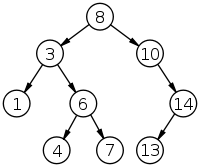
\includegraphics[width=.5\textwidth]{Binarysearchtree.png}

\begin{flushright}
(Wikipedia)
\end{flushright}

\end{frame}

\begin{frame}[fragile]
\frametitle{Binary Search Tree Interface}

\begin{itemize}
\item constructor: creates empty tree
\item insert(value): inserts elements
\item find(value) $\to$ boolean
\item size() $\to$ number
\item remove(value): removes a value
\end{itemize}
\end{frame}

\begin{frame}[fragile]
\frametitle{Defensive Programming}

Defensive programming means writing code that will catch bugs early.
\end{frame}

\begin{frame}[fragile]
\frametitle{Assertions}
\begin{python}
def stddev(values):
    '''
    S = stddev(values)

    Compute standard deviation
    '''
    assert len(S) > 0, 'stddev: got empty list.'
    ...
\end{python}
\end{frame}

\begin{frame}[fragile]
\frametitle{Assertions}

\begin{python}
def stddev(values):
    '''
    S = stddev(values)

    Compute standard deviation
    '''
    if len(S) <= 0:
        raise AssertionError(
            'stddev: got empty list.')
    ...
\end{python}

\end{frame}

\begin{frame}[fragile]
\frametitle{}

\begin{python}
def factorial(N):
    '''
    fN = factorial(N)

    Returns the factorial of N.

    N must be equal or greater than zero.
    '''
    if N == 0:
        return 1.
    return N * factorial(N-1)
\end{python}
\end{frame}

\begin{frame}[fragile]
\frametitle{Preconditions}

\begin{quote}
In computer programming, a precondition is a condition or predicate that must always be true just prior to the execution of some section of code.
\end{quote}

\begin{flushright}
(Wikipedia)
\end{flushright}

\end{frame}

\begin{frame}[fragile]
\frametitle{Preconditions}
\begin{block}{Other Languages}
\begin{itemize}
\item \alert{C/C++} \lstinline{#include <assert.h>}
\item \alert{Java} \lstinline{assert }\textit{pre-condition}
\item \alert{Matlab} \lstinline{assert()} (in newer versions)
\item \alert{\ldots} \ldots
\end{itemize}
\end{block}
\end{frame}

\begin{frame}[fragile]
\frametitle{Assertions Are Not Error Handling!}

\begin{itemize}
\item Error handling protect against outside events.
\item Assertions \alert{should never} be false.
\end{itemize}
\end{frame}

\begin{frame}[fragile]
\frametitle{Programming by Contract}
\begin{enumerate}
\item pre-conditions.
\item post-conditions.
\item invariants.
\end{enumerate}
\end{frame}

\begin{frame}[fragile]

\begin{block}{Pre-condition}
What must be true before calling a function.
\end{block}

\begin{block}{Post-condition}
What is true after calling a function.
\end{block}
\end{frame}

\begin{frame}[fragile]
\frametitle{Pre-conditions}

\begin{block}{Examples}
\begin{itemize}
\item sort: element must be comparable.
\item BST.add(val): element must be comparable to all elements in BST.
\item BST.find(val): element must be comparable to all elements in BST.
\item \ldots
\end{itemize}
\end{block}
\end{frame}

\begin{frame}[fragile]
\frametitle{Post-conditions}

\begin{block}{Examples}
\begin{itemize}
\item \lstinline{sort}: elements are in sorted order.
\item \lstinline{BST.add(val)}: value is in tree.
\item \lstinline{BST.remove(val)}: value is not in tree.
\item \ldots
\end{itemize}
\end{block}
\end{frame}

\begin{frame}[fragile]
\frametitle{Invariants}
Invariants make sense within the context of related functions.
\end{frame}

\begin{frame}[fragile]
\begin{block}{Bacteria class}
\begin{itemize}
\item \lstinline{sigma >= 0}
\end{itemize}
\end{block}

\begin{block}{Binary Search Tree}
\begin{itemize}
\item Items in left sub-tree are smaller than cur item.
\item Items in right sub-tree are bigger than cur item.
\item All items are comparable.
\end{itemize}
\end{block}
\end{frame}

\begin{frame}[fragile]
\frametitle{Testing}

Do you test your code?

\end{frame}

\begin{frame}[fragile]
\frametitle{Unit Testing}

\begin{python}
def test_stddev_const():
    assert stddev([1]*100) < 1e-3

def test_stddev_positive():
    assert stddev(range(20)) > 0.
\end{python}

\end{frame}

\begin{frame}[fragile]
\frametitle{Nosetest}

Nose software testing framework:
\begin{itemize}
\item Tests are named \lstinline{test_}\textit{something}.
\item Conditions are \lstinline{assert}ed.
\end{itemize}

\end{frame}

\begin{frame}[fragile]
\frametitle{Software Testing Philosophies}

\begin{enumerate}
\item Test everything. Test it twice.
\item Write tests first.
\item Regression testing.
\end{enumerate}
\end{frame}

\begin{frame}[fragile]
\frametitle{Regression Testing}

Make sure bugs only appear once!

\end{frame}

\begin{frame}[fragile]

\centering
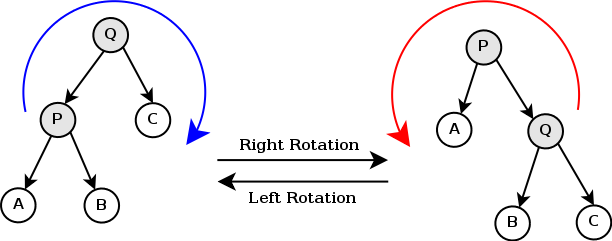
\includegraphics[width=.9\textwidth]{Treerotation}

\begin{flushright}
(Wikipedia)
\end{flushright}
\end{frame}



\end{document}
